\section{IAmMuse Response Times}
\label{section: evaluation - response times}

This section analyses the \textit{response time} of the different systems.
The response time is the delay, in frames, between the ground truth changing and the prediction model correctly predicting the new state.
The response times of the \textit{MARS baseline}, \textit{pre-trained} or \textit{full calib} models have been excluded, as their low classification accuracy makes this information statistically uninformative.
The response times displayed are thus for the \textit{MARS partial standard} recording, as it had the highest classification accuracy, and because the results for \textit{MARS partial standard} and \textit{standard to free} were very similar.
However, the high variance in the output of the \textit{MARS partial standard} model artificially deflates its average response time.
Since the metric considers the \textit{first correct frame} as a successful response, the rapid change of predictions means that the model can at times achieve low latency scores, because it rapidly switches state, and not because it detected the changing input data correctly.

The response times of both IAmMuse and MARS are shown in \cref{fig: response delay}.
Each bar represents the number of state changes which were recognised in that precise number of frames.
\Cref{fig: cumulative response likelihood} shows the cumulative response likelihood, the number of frames it took until a response was measured.
These figures show that IAmMuse produces a correct response within a single frame in 36\% of state changes, while MARS does so in 51\%.
After seven frames, IAmMuse will have produced a correct response in 50\% of cases, while it takes until nearly 30 frames to produce a correct response in 80\% of cases.
% \ednote{Explain this in more detail}
MARS's response time is lower than that of IAmMuse, though this may in part be due to the high variance in its output.
The rapidly changing predictions of MARS will allow it to receive \textit{low response times} coincidentally, as opposed to achieving low response times through genuine state detection.
This happens because the response time metric only considers the time until the \textbf{first} successful prediction.
% Since the response time metric only considers the first successful prediciton, the high variance in the output will 

% However, the lower response times may in part be caused by the high variance of the MARS model.
% Because the response time metric measures the delay until the first successful prediction, the MARS model's tendency to rapidly switch states allows it to achieve low latency scores coincidentally, rather than through accurate tracking of the input data.


\begin{figure}[!htb]
    \makebox[\textwidth][c]{
    \begin{subfigure}[t]{0.66\textwidth}
        \centering
        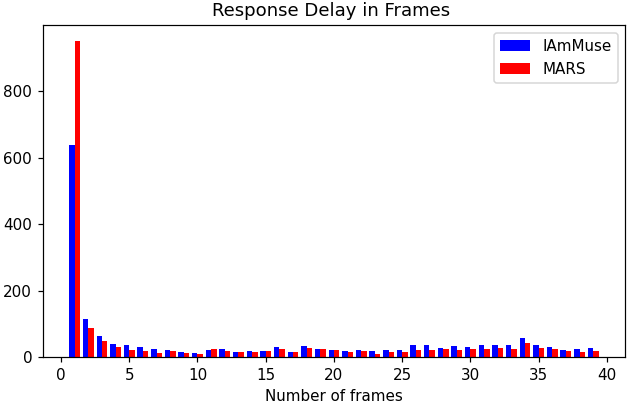
\includegraphics[width=\linewidth]{figures/results/response delay.png}
        \caption{Response delay of IAmMuse (blue) and MARS (red)}
        \label{fig: response delay}
    \end{subfigure}
    \hspace{0.5cm}
    \begin{subfigure}[t]{0.66\textwidth}
        \centering
        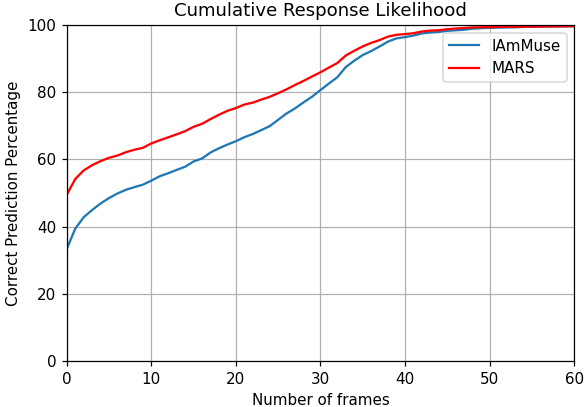
\includegraphics[width=\linewidth]{figures/results/cumulative response likelihood.png}
        \caption{Cumulative response likelihood of IAmMuse (blue) and MARS (red)}
        \label{fig: cumulative response likelihood}
    \end{subfigure}
    }
    \caption{Response characteristics of IAmMuse and MARS}
\end{figure}

